\documentclass[12pt,a4paper]{scrartcl}
\usepackage[utf8]{inputenc}
\usepackage{graphicx}
\usepackage{ngerman}
\usepackage{url}
\usepackage{amsmath}
\usepackage{caption}
\usepackage{wrapfig}
\usepackage{eurosym}
\usepackage{biblatex}
\usepackage{url}
\usepackage{color}
\usepackage{listings}
\usepackage{hyperref}
\usepackage[table]{xcolor}
\linespread{1.4}

\definecolor{mygreen}{rgb}{0,0.6,0}
\definecolor{mygray}{rgb}{0.5,0.5,0.5}
\definecolor{mylightgray}{rgb}{0.7,0.7,0.7}
\definecolor{mylightergray}{rgb}{0.9,0.9,0.9}
\definecolor{mymauve}{rgb}{0.58,0,0.82}

\let\origitemize\itemize
\def\itemize{\origitemize\itemsep0pt}

\lstset{ 
  backgroundcolor=\color{white},   
  basicstyle=\ttfamily\footnotesize,          
  breakatwhitespace=false,         
  breaklines=true,  
  commentstyle=\color{mygreen}, 
  escapeinside={\%*}{*)}, 
  extendedchars=true,             
  keepspaces=true,                 
  keywordstyle=\color{blue},
  language=Octave,
  numbers=left,                   
  numbersep=15pt,                  
  numberstyle=\tiny\color{mygray}, 
  showspaces=false,                
  showstringspaces=false,          
  showtabs=false,                  
  stringstyle=\color{mymauve},
  tabsize=2,
  title=\lstname,
  captionpos=b
}

\renewcommand*\lstlistingname{Codebeispiel}    %Rename Listings

\renewcommand*\thesection{\arabic{section}}

\makeatletter
\renewcommand\subparagraph{\@startsection{subparagraph}{5}{\parindent}%
    {3.25ex \@plus1ex \@minus .2ex}%
    {0.75ex plus 0.1ex}% space after heading
    {\normalfont\normalsize\bfseries}}
\makeatother

\begin{document}
\title{Praktikum Data Mining}
\subtitle{Energieverbrauch und CO2-Emmisionen \newline Vorhersage und Clustering auf Finanzdaten}
\author{Oliver Fesseler \and Maria Florus\ss \and Stefan Seibert \and  Daniel Grie\ss haber}
\maketitle
\newpage
\tableofcontents
\newpage

\part*{Energieverbrauch und CO\textsubscript{2}-Emmission}

\section*{Datenverwaltung und Statistik}
\subsection*{Einlesen der Daten, Hinzuf\"ugen der GPS Koordinaten, Abspeichern in neuer Datei}
Bei der Umsetzung der Aufgaben haben wir mit verschiedenen Darstellungsformen der Daten experimentiert. Im ersten Plot fallen vor allem die Vielverbraucher einzelner Energieformen auf. Beim zweiten Plot k\"onnen die verschiedenen Energiemixe pro Land direkt miteinander verglichen werden, da sie alle im selben Ma\ss stab nebeneinander dargestellt werden.

\subparagraph{ Ausgehend von der implementierten Visualisierung des Energieverbrauchs der L\"ander: Nennen Sie die 3 Ihrer Meinung nach interessantesten Beobachtungen.}

\begin{enumerate}
\item Durch die wenigen Industriel\"ander mit signifikant h\"oherem Energieverbrauch, wie China oder die USA, wird der Plot so verzerrt, dass die L\"ander mit durchschnittlichem Verbrauch im Plot so gestaucht werden, dass sie kaum zu erkennen sind. Dies k\"onnte behoben werden, wenn die Daten mit den Einwohnerzahlen aller L\"ander normalisiert werden w\"urden. So k\"onnte der Pro-Kopf-Verbrauch berechnet werden, was einen besseren Vergleich der einzelnen L\"ander bietet.
\item Dieses Prinzip wird klar bei der Betrachtung von China und Indien, die von der Einwohnerzahl her vergleichbar sind (China 1,3 Mrd., Indien 1,2 Mrd.\footnote{Stand 2012, Quelle: Wikipedia}). China zeigt einen weitaus h\"oheren Verbrauch als Indien an den in beiden L\"andern h\"aufigen Energieformen Kohle und \"Ol.
Zus\"atzlich w\"aren noch andere Normalisierungsfaktoren interessant:
\begin{itemize}
\item Bruttoinlandsprodukt
\item Au\ss enhandelsstatistik oder Export der L\"ander in US\$
\item Technologieindex
\end{itemize}
\item Die zwei L\"ander mit dem h\"ochsten Energieverbrauch sind China und die USA. Dies f\"allt bei der Betrachtung des Gesamtenenergieverbrauchs auf. Bei der Betrachtung des Verbrauchs einzelner Energieformen wirkt es als sei China durch seinen hohen Kohleverbrauch weit vor den USA.
\end{enumerate}

\subparagraph{Abgabe: Relevante Dateien}
\begin{itemize}
\item \lstinline{energy_consumption_per_country.py} und \lstinline{energy_consumption_per_country_V2.py} \\- Implementierung Aufgabe 2.1.2: 1) - 2)
\item \lstinline{energy_consumption_per_country.pdf} \\- Ausgabe des Skripts \lstinline{energy_consumption_per_country.py} 
\item \lstinline{energy_consumption_per_country_V2.pdf} \\- Ausgabe des Skripts \lstinline{energy_consumption_per_country_V2.py}
\item \lstinline{appendGeoCoordinates.py} \\- Implementierung Aufgabe 2.1.2: 3) - 5)
\item \lstinline|EnergyMixGeo.csv|  \\- Ausgabe des Skripts \lstinline{appendGeoCoordinates.py}
\end{itemize}





\subsection*{Statistik der Daten}

\subparagraph{Erkl\"aren Sie s\"amtliche Elemente eines Boxplot (allgemein). }
\begin{figure}[!h]
\centering
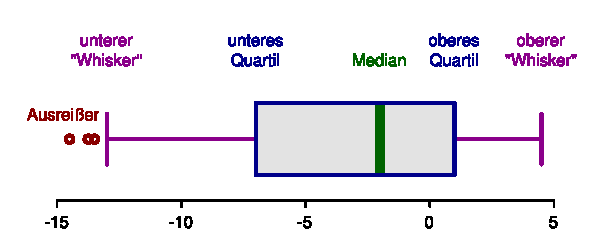
\includegraphics[width=0.7\textwidth]{Plots/Elements_of_a_boxplot.pdf}
\end{figure}
\begin{itemize}
\item Ausrei\ss er (\grqq Outliers\grqq ), in Python mit 'sym' zu setzen. \\
Daten die au\ss erhalb der Whisker liegen und somit als Ausrei\ss er deklariert werden.
\item Whisker, L\"ange in Python mit 'whis' zu setzen.\\
Standartm\"a\ss ig die 1,5-fache L\"ange des entsprechenden Quartils. 
\item Quartil\\
Die Quartile sind Bestandteile der Box, welche 50 \% aller Daten enth\"alt. Dabei enth\"alt das obere Quartil, die 25\%, die \"uber dem Median, das untere Quartil, die 25\%, die unter dem Median liegen.
\item Median\\
Der mittlere Wert (nicht Mittelwert oder Durchschnitt), der aus dem gesamten Datensatz ermittelt wird. Er teilt den Boxplot in zwei H\"alften, die wiederum jeweils in Whisker und Quartil unterteilt werden.
\end{itemize}

\subparagraph{Diskutieren Sie die im Boxplot angezeigte Statistik der Energieverbrauchdaten.}
\begin{itemize}
\item Durch den signifikant h\"oheren Verbrauch von China und den USA wird beim Anzeigen der Ausrei\ss er der restliche Boxplot soweit gestaucht, dass vern\"unftigen Daten mehr abgelesen werden k\"onnen. 
Um die Verteilung innerhalb der verschiedenen Boxplots besser vergleichen zu k\"onnen, entschlossen wir uns au\ss erdem jede Energieform in einem einzelnen Subplot darzustellen. 
\item Im Gesamtplot lassen sich die einzelnen Energieformen gut miteinander vergleichen, in den einzelnen Plots k\"onnen die Verteilungen innerhalb der Plots besser dargestellt werden.  
\item Beim Boxplot der nuklearen Energieform f\"allt auf, dass der Median samt unterem Quartil und unterem Whisker auf 0 liegt. Dies liegt daran, dass weniger als die H\"alfte aller L\"ander nukleare Energie verwenden. 
\item Im Gesamtplot kann man erkennen, dass \"Ol die einzige Energieform ist, deren unterer Whisker nicht auf 0 liegt. Also verwendet jedes in Betracht gezogene Land \"Ol. Jede andere Energieform wird von mindestens einem Land nicht verwendet. 
\end{itemize}

\subparagraph{Abgabe: Relevante Dateien}
\begin{itemize}
\item \lstinline{enegryStatistics.py} \\- Implementierung Aufgabe 2.1.3: 1) - 3)
\item \lstinline{energyconsumption_by_energyform_in_seperate_subboxplots.pdf} und \\ \lstinline{energyconsumption_by_energyform_in_one_plot.pdf} \\- Ausgabe des Skripts \lstinline{enegryStatistics.py}
\end{itemize}


\section*{Anwendung von Verfahren des un\"uberwachten Lernens auf Energieverbrauchsdaten}

\subsection*{Hierarchisches Clustering}
\subparagraph{Was wird beim Standardisieren gemacht? Welcher Effekt k\"onnte ohne Standardisieren beim Clustering eintreten (insbesondere wenn die euklidische Metrik verwendet wird)?}

\textbf{Antwort:}

\subparagraph{Welches Land ist bez\"uglich des Verbrauchs der hier betrachteten Energiequellen Deutschland am \"ahnlichsten, wenn f\"ur die linkage-method \lstinline{average} und die Metrik \lstinline{correlation} konfiguriert wird?}

\textbf{Antwort:} Belgien


\end{document}